\chapter{System Modelling}
With the given setup \fxnote{Fix this once we have agreed on a name for the cubli thingy} being described, it is necessary to study its natural behavior in more details by deriving a model of this system. This chapter shows the process used to put up this model and an analysis of its pertinence. With this model, it shall be possible to determine realistic requirements for the controllers to implement in this project, see \chapref{chap:specifications}.

As a start to this modelling, a mechanical drawing of the Cubli showing angles and coordinate system conventions is seen in \figref{cubliMechanical}. A two-dimensional global coordinate system is chosen with its origin on the pivot point of the frame. Moreover, angles of the total body and the wheel count grow clockwise.

\begin{figure}[H]
 \centering
 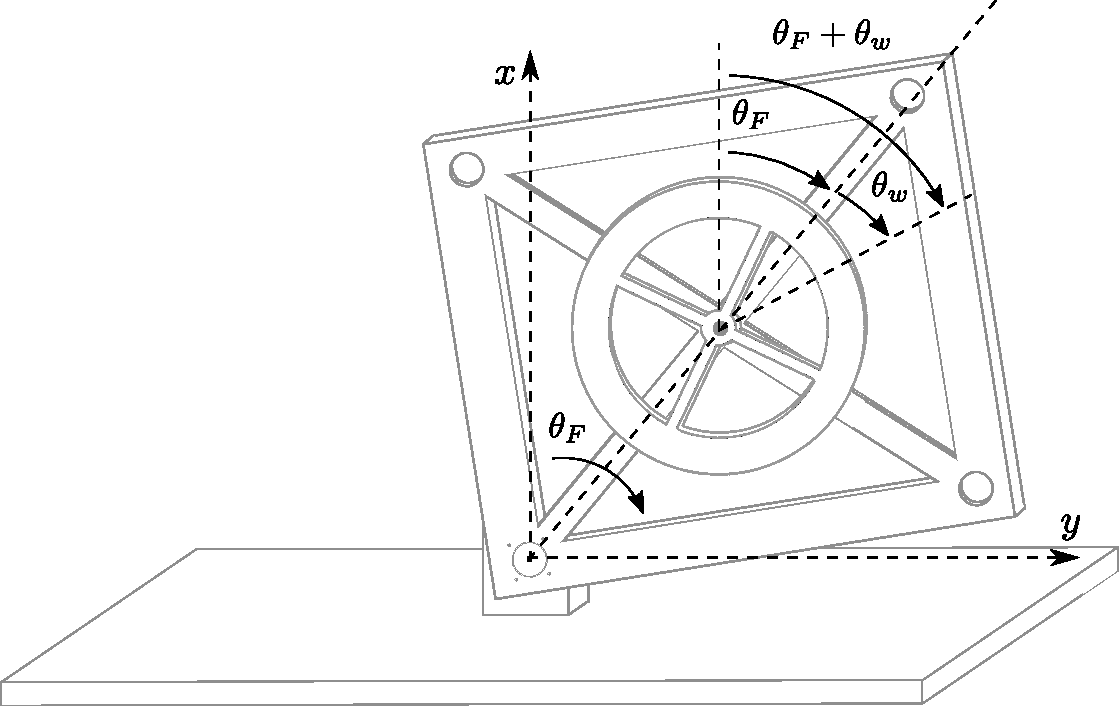
\includegraphics[scale=0.6]{figures/mechanicalSystem}
 \caption{Mechanical drawing of the Cubli, including angle coordinate system conventions}
 \label{cubliMechanical}
\end{figure}

%As shown in \figref{cubliMechanical}, 
In the next section, a complete model of the given setup is derived from Newton's Second Law of motion and rotation.